\section{Analyse des Schmalbandinterferogramms}
Der Wellenl�ngenbereich des Muffelofen wird mit einem Schmalbandfilter reduziert. Da durch die Filterung auch die Intensit�t verringert wird, muss die Verst�rkung des Log-In-Verst�rkers korrigiert werden. Aufgrund des Filters wird eine ged�mpfte Cosinus-Schwingung symmetrisch um den Wei�lichtpunkt des Muffelofen erwartet. Aus dem aufgenommen Interferogramm soll die Wellenl�nge der maximalen Transmission und die Breite des 1/e-Abfalls der Einh�llenden bestimmt werden. Mit diesen beiden Werten kann die Breite des Schmalbandfilters bestimmt werden.
Das Interferogramm ist in Abbildung \ref{fig:filter_weiss} zu sehen. 

\begin{figure}[H]
\centering
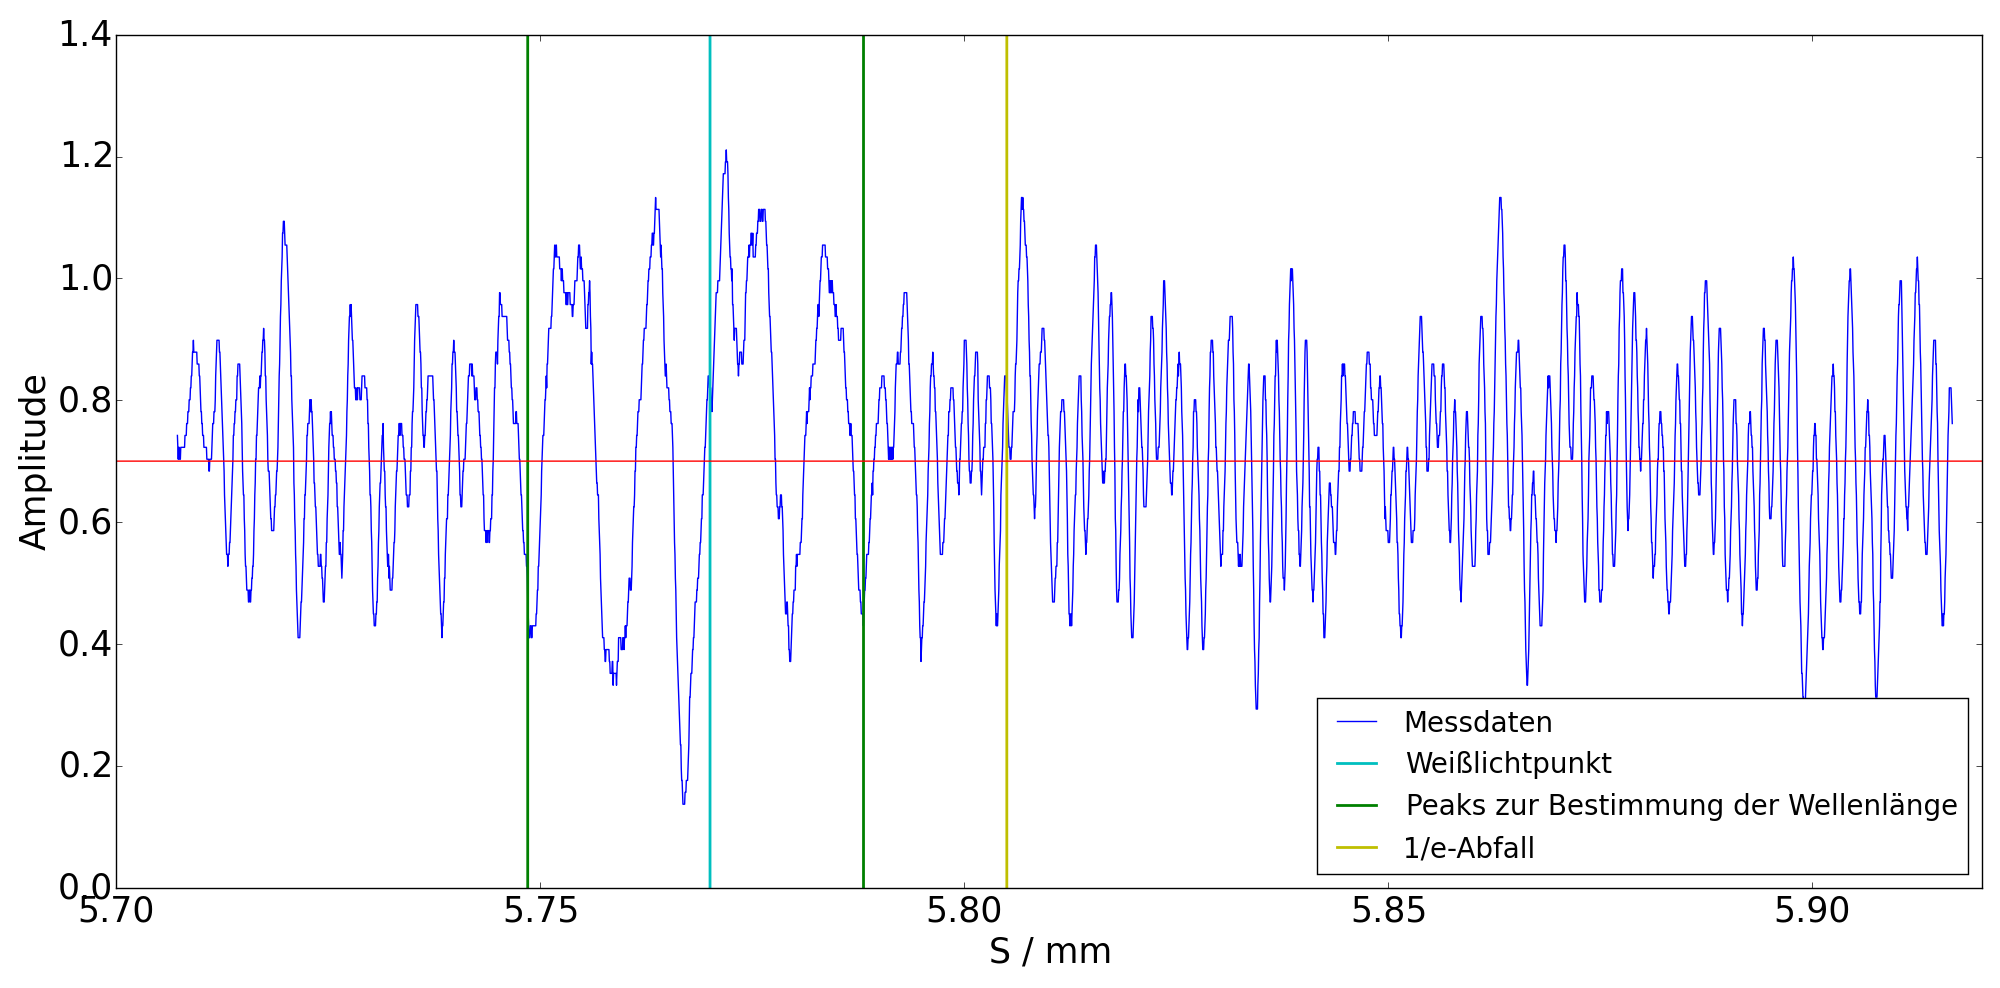
\includegraphics[scale = 0.32]{filter_weiss.png}
\caption{Interferogramm f�r den Muffelofen mit Schmalbandfilter. Die gr�nen Linien markieren den Bereich f�r die Bestimmung der Wellenl�nge, die rote Linie markiert die Nulllage}
\label{fig:filter_weiss}
\end{figure}

Aus den Interferrogramm ergeben sich die Werte in Tabelle \ref{tab:parameter_filter}. Es wurde ein kleines Intervall um den Wei�lichtpunkt gew�hlt, da in diesem Bereich die Abst�nde zwischen den Peaks regelm��ig sind. Aus den Werten ergibt sich eine Wellenl�nge von 2.91(5)$\mu$m, dieser Wert weicht um 39,82\% vom Literaturwert von 3,31$\mu$m ab (Quelle:\cite{Staatsex_Michels}). Mit diesem Wert l�sst sich der Parameter b aus Gleichung \ref{eqn:B_schmalband} bestimmten.

\begin{align}
b = \frac{2 \pi}{\lambda} = 1.988(3) \frac{1}{\mu m}
\end{align}

\begin{table}[H]
\centering
\caption{Messwerte f�r die Bestimmung der Wellenl�nge des Wei�lichtpunkts}
\label{tab:parameter_filter}
\begin{tabular}{|c|c|c|c|}
\hline x$_1$ / mm & x$_2$ / mm & s / mm & n \\ 
\hline 5,7485(3) & 5,7881(3) & 0,0396(4) & 5 \\ 
\hline 
\end{tabular} 
\end{table}

F�r die Bestimmung des 1/e-Abfalls wird die Position des Wei�lichtpunkts verwendet. Die Amplitude am Wei�lichtpunkt betr�gt ca. 0,57 V. Das Minimum des Interferogramms liegt bei ca. 0,4. Der 1/e-Abfall ergibt sich bei einer Position von 5.805(3) $\mu$m mit einer Amplitude von 0,208 V erreicht. Dadurch ergibt sich eine Breite des 1/e-Abfalls von 0,35(2) mm. Aus den Werten l�sst sich die spektrale Verteilung des Ofens bestimmen. Die Wellenzahlen ergeben sich mit: 

\begin{align}
\bar{\nu_1} = b - \frac{2}{a} = 1,93(4) \mu m^{-1}\\
\bar{\nu_2} = b - \frac{2}{a} = 2,04(4) \mu m^{-1}
\end{align}

Aus den beiden Werten l�sst sich nach \cite{Staatsex_Michels} die e$^{-1}$-Breite $\Delta \lambda$ des Schmalbandfilters bestimmen.

\begin{align}
\Delta \lambda = \frac{1}{\bar{\nu_1}} - \frac{1}{\bar{\nu_2}}= 0,289(8) \mu m
\end{align}

Erwartet wurde ein Wert von 0,060 $\mu$m \cite{Staatsex_Michels}. Der Bestimmte Wert liegt ca. eine Gr��enordnung �ber halb des theoretischen Wertes, dies kommt wahrscheinlich von dem ungenau bestimmten a. 

Aus den beiden Parametern a und b ergibt sich die spektrale Verteilung des Muffelofen in Abbildung \ref{fig:spektrum_filter}.

\begin{figure}[H]
\centering
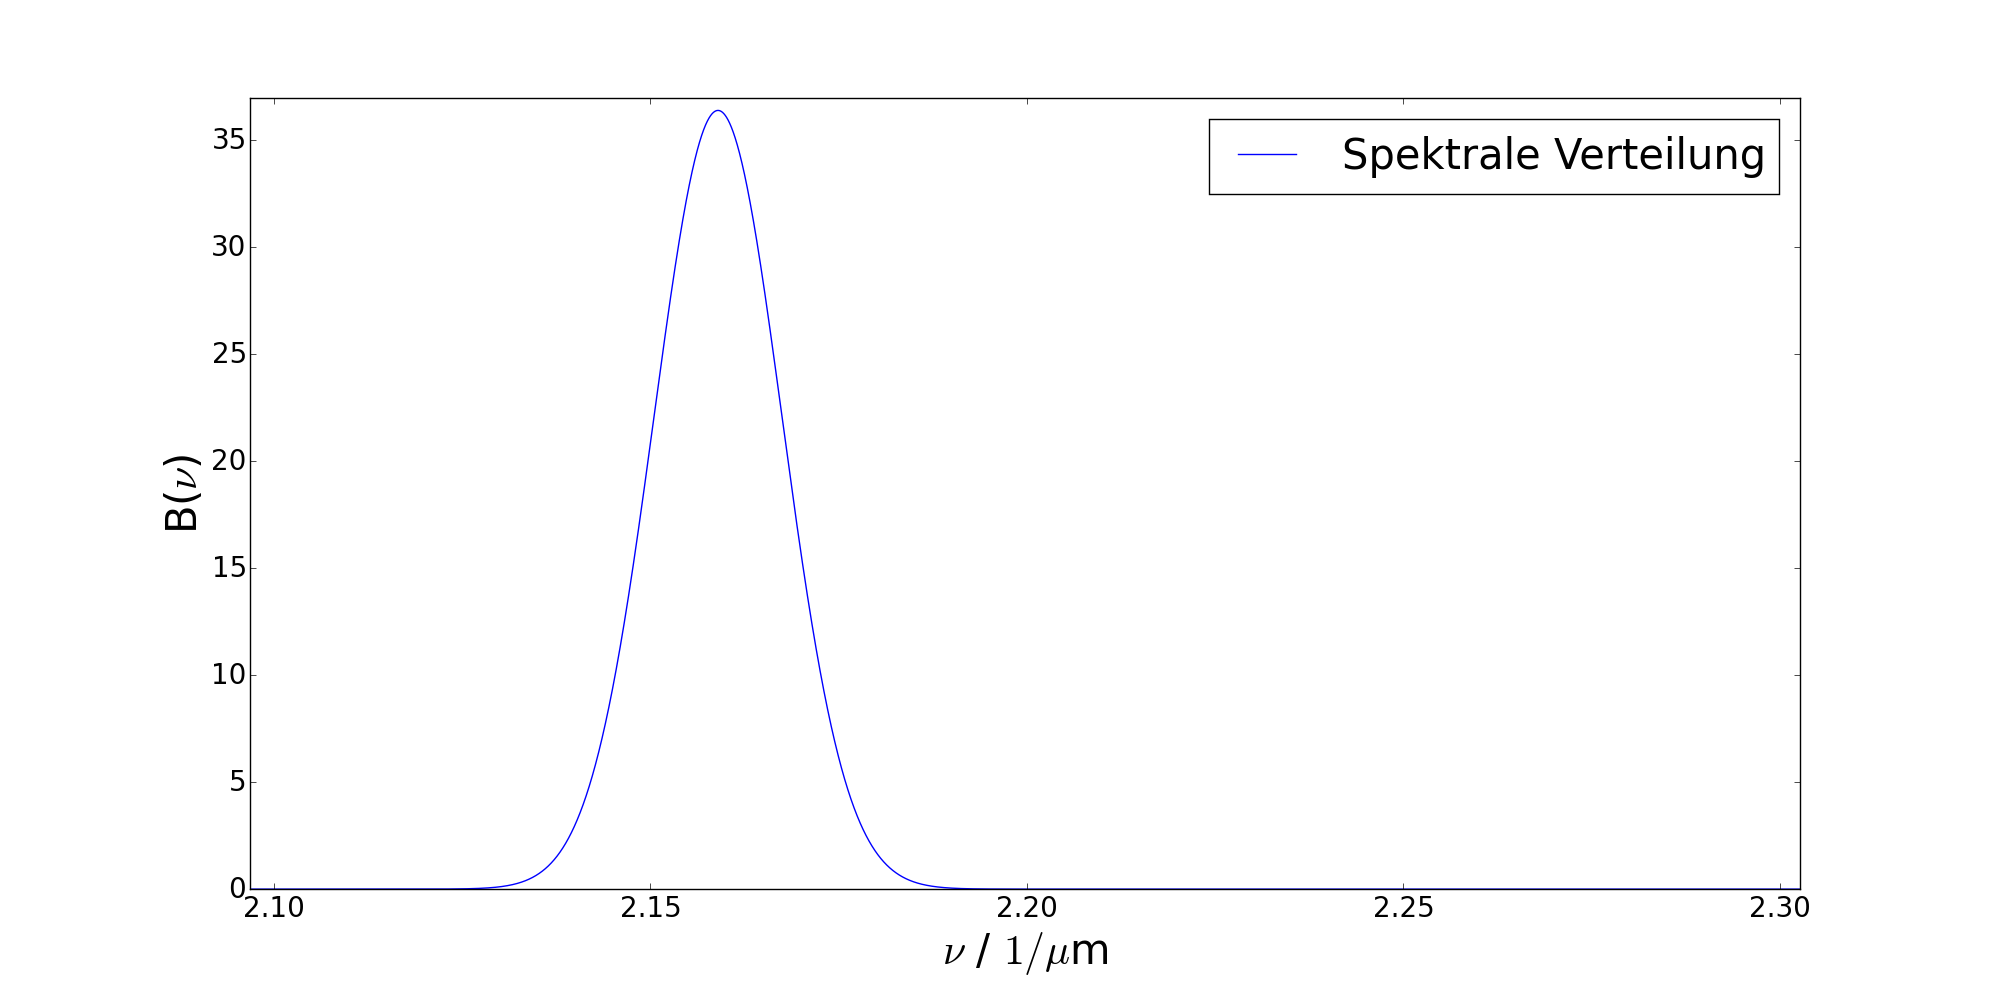
\includegraphics[scale = 0.33]{verteilung_filter.png}
\caption{Spektrale Verteilung des Schmalbandfilters}
\label{fig:spektrum_filter}
\end{figure}

Zum Schluss soll erw�hnt werden, dass bei Anwendung einer FFT, eines Algorithmusses f�r die diskrete Fouriertransformation, ein �hnliches Ergebnis zustande kommt. Da die FFT f�r periodische Signale geeignet ist, kann zur Rauschunterdr�ckung eine sogenannte Fensterfunktion verwendet werden, welche das Signal 'sanft' ein und ausblendet. Das FFT-Spektrum ohne Fensterfunktion ist in Abbildung \ref{fig:fftfilterinterferogramm_ohne_fenster} dargestellt.
\begin{figure}[H]
\centering
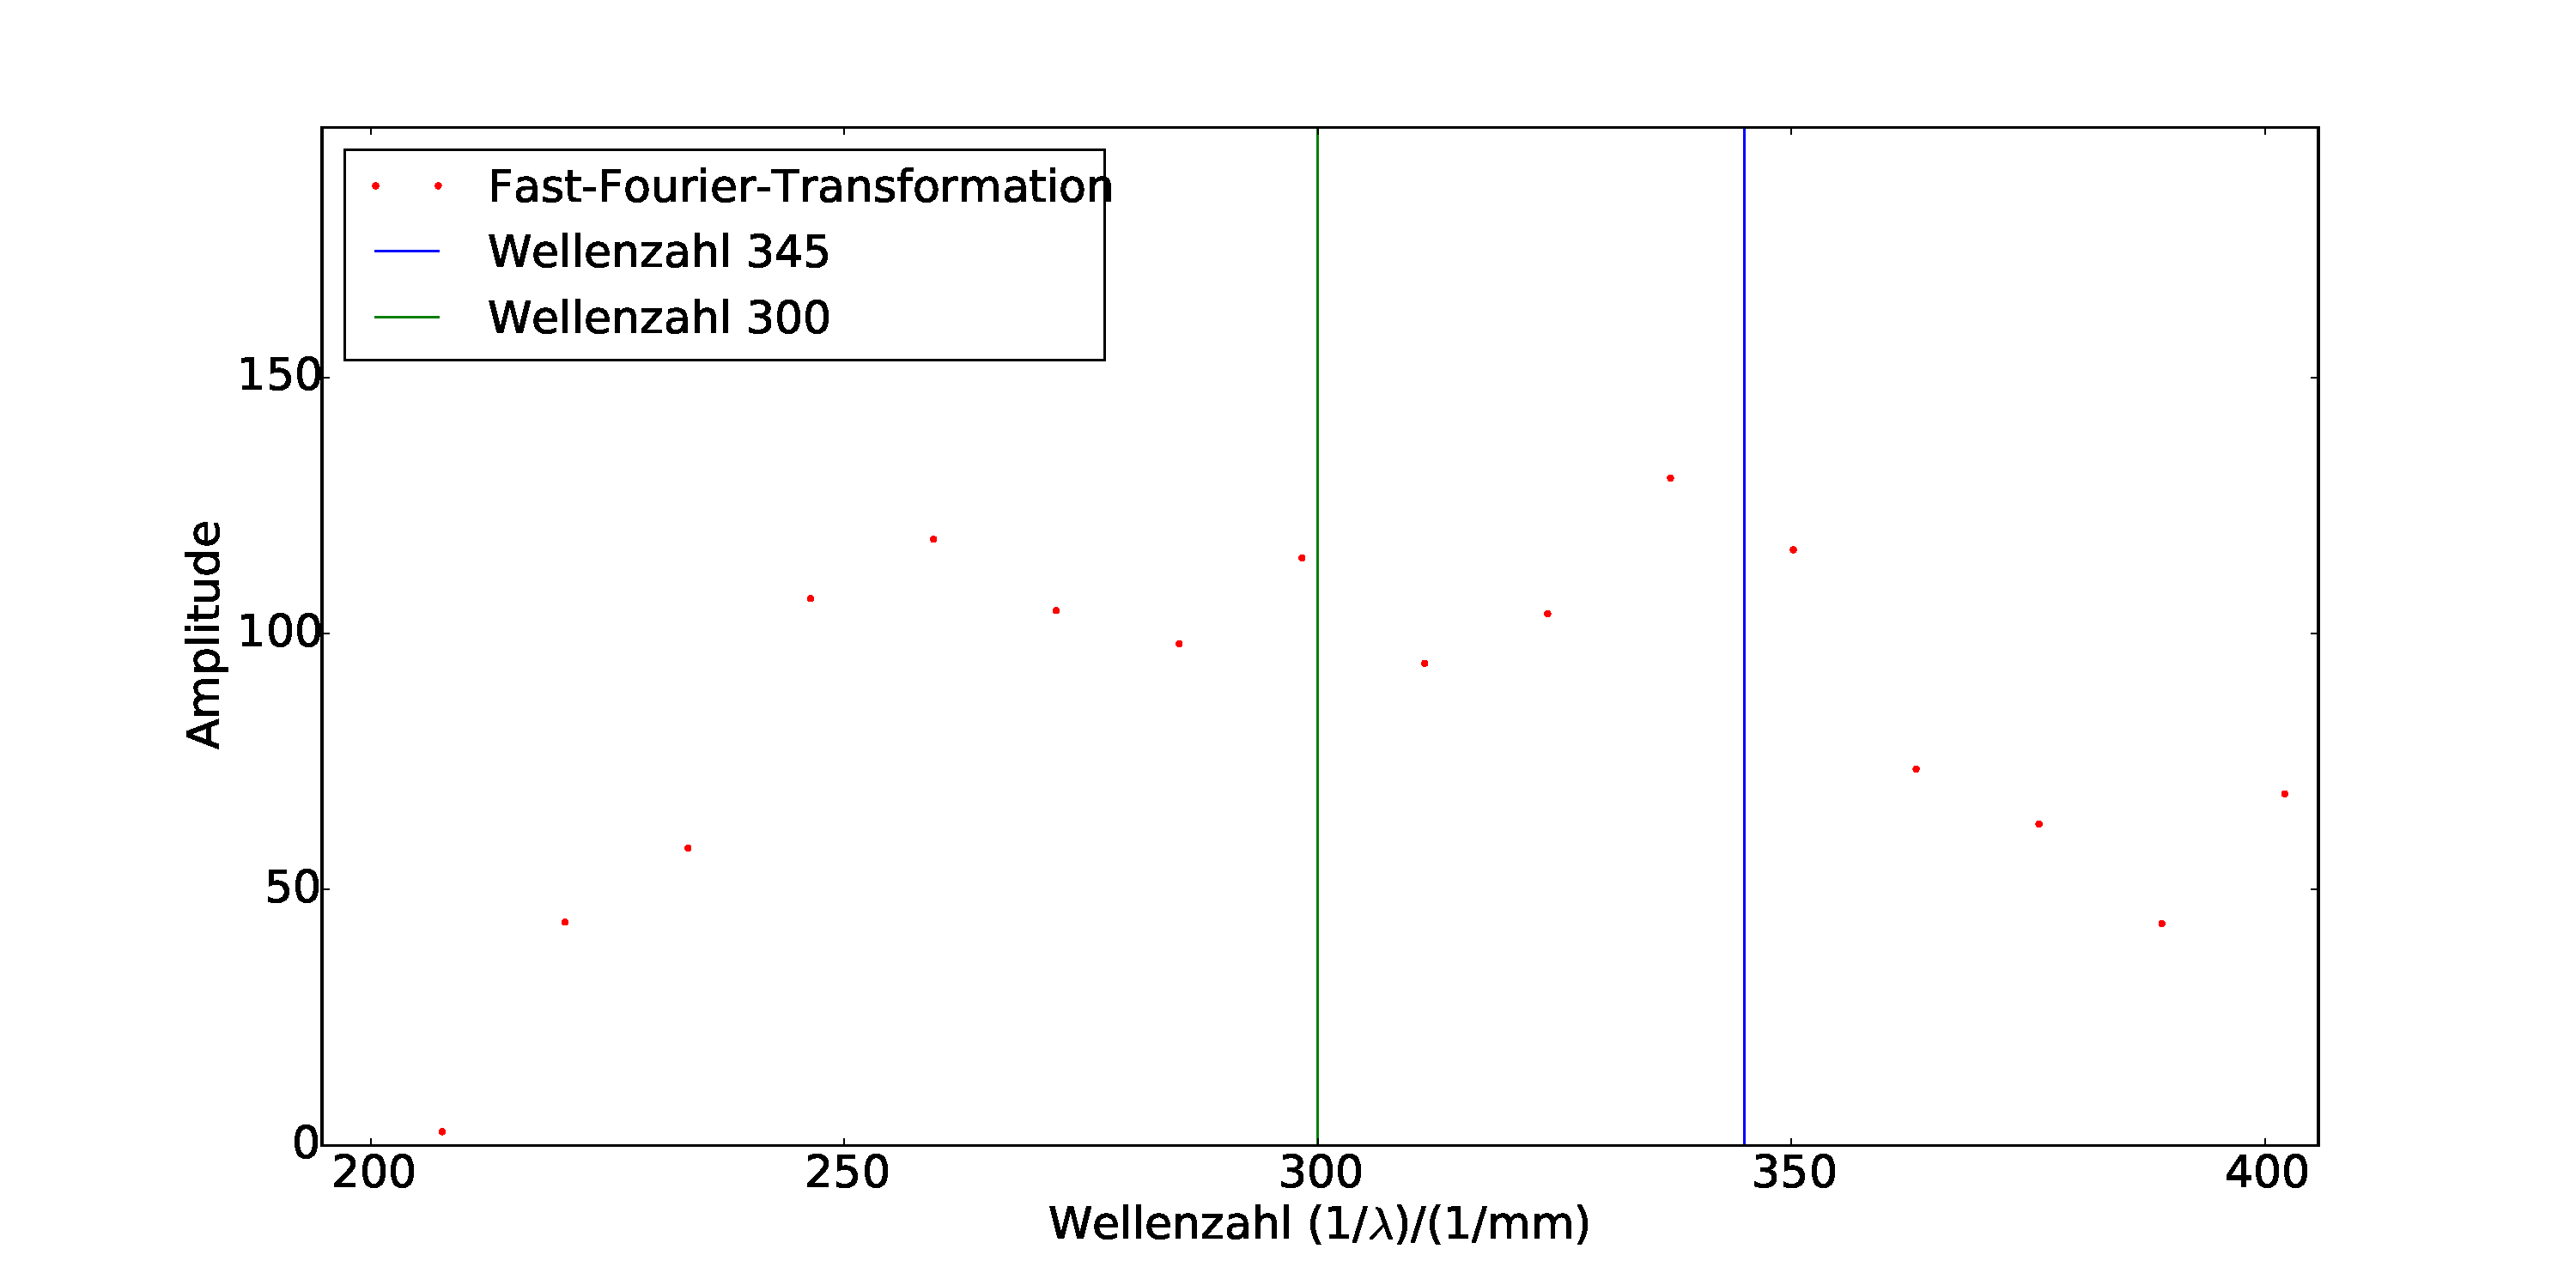
\includegraphics[scale = 0.38, clip = true, trim = 3cm 0cm 3cm 0cm]{Wellenzahlen200-400FilterohneFenster}
\caption{Diskrete Fouriertransformation des Filterinterferogramms f�r Wellenzahlen ($1/\lambda$) von \SI{200}{$\frac{1}{mm}$} bis \SI{400}{$\frac{1}{mm}$}  ohne Fensterfunktion (verrauscht)}
\label{fig:fftfilterinterferogramm_ohne_fenster}
\end{figure}
Man sieht, dass die Wellenzahl \SI{300(2)}{$\frac{1}{mm}$} im Spektrum vertreten ist, welche einer Wellenl�nge von \SI{3,33(2)}{$\mu$m} entspricht. Beim ein und Ausblenden des Signals mit den Funktionen $f(x)=(\frac{1-\cos(\frac{2 \pi x}{L})}{2})$ und $f(x)=(\frac{1-\cos(\frac{2 \pi x}{L})}{2})^4$, um das Rauschen durch die Nichtperiodizit�t zu unterdr�cken, wird diese Wellenzahl jedoch herausgefiltert. Die beiden Spektren, welche durch Anwendung der beiden Filterfunktionen entstehen, sind in den Abbildungen \ref{fig:fftfilterinterferogramm_k_1} und \ref{fig:fftfilterinterferogramm_k_4} dargestellt.
\begin{figure}[H]
\begin{subfigure}[t]{0.49\textwidth}
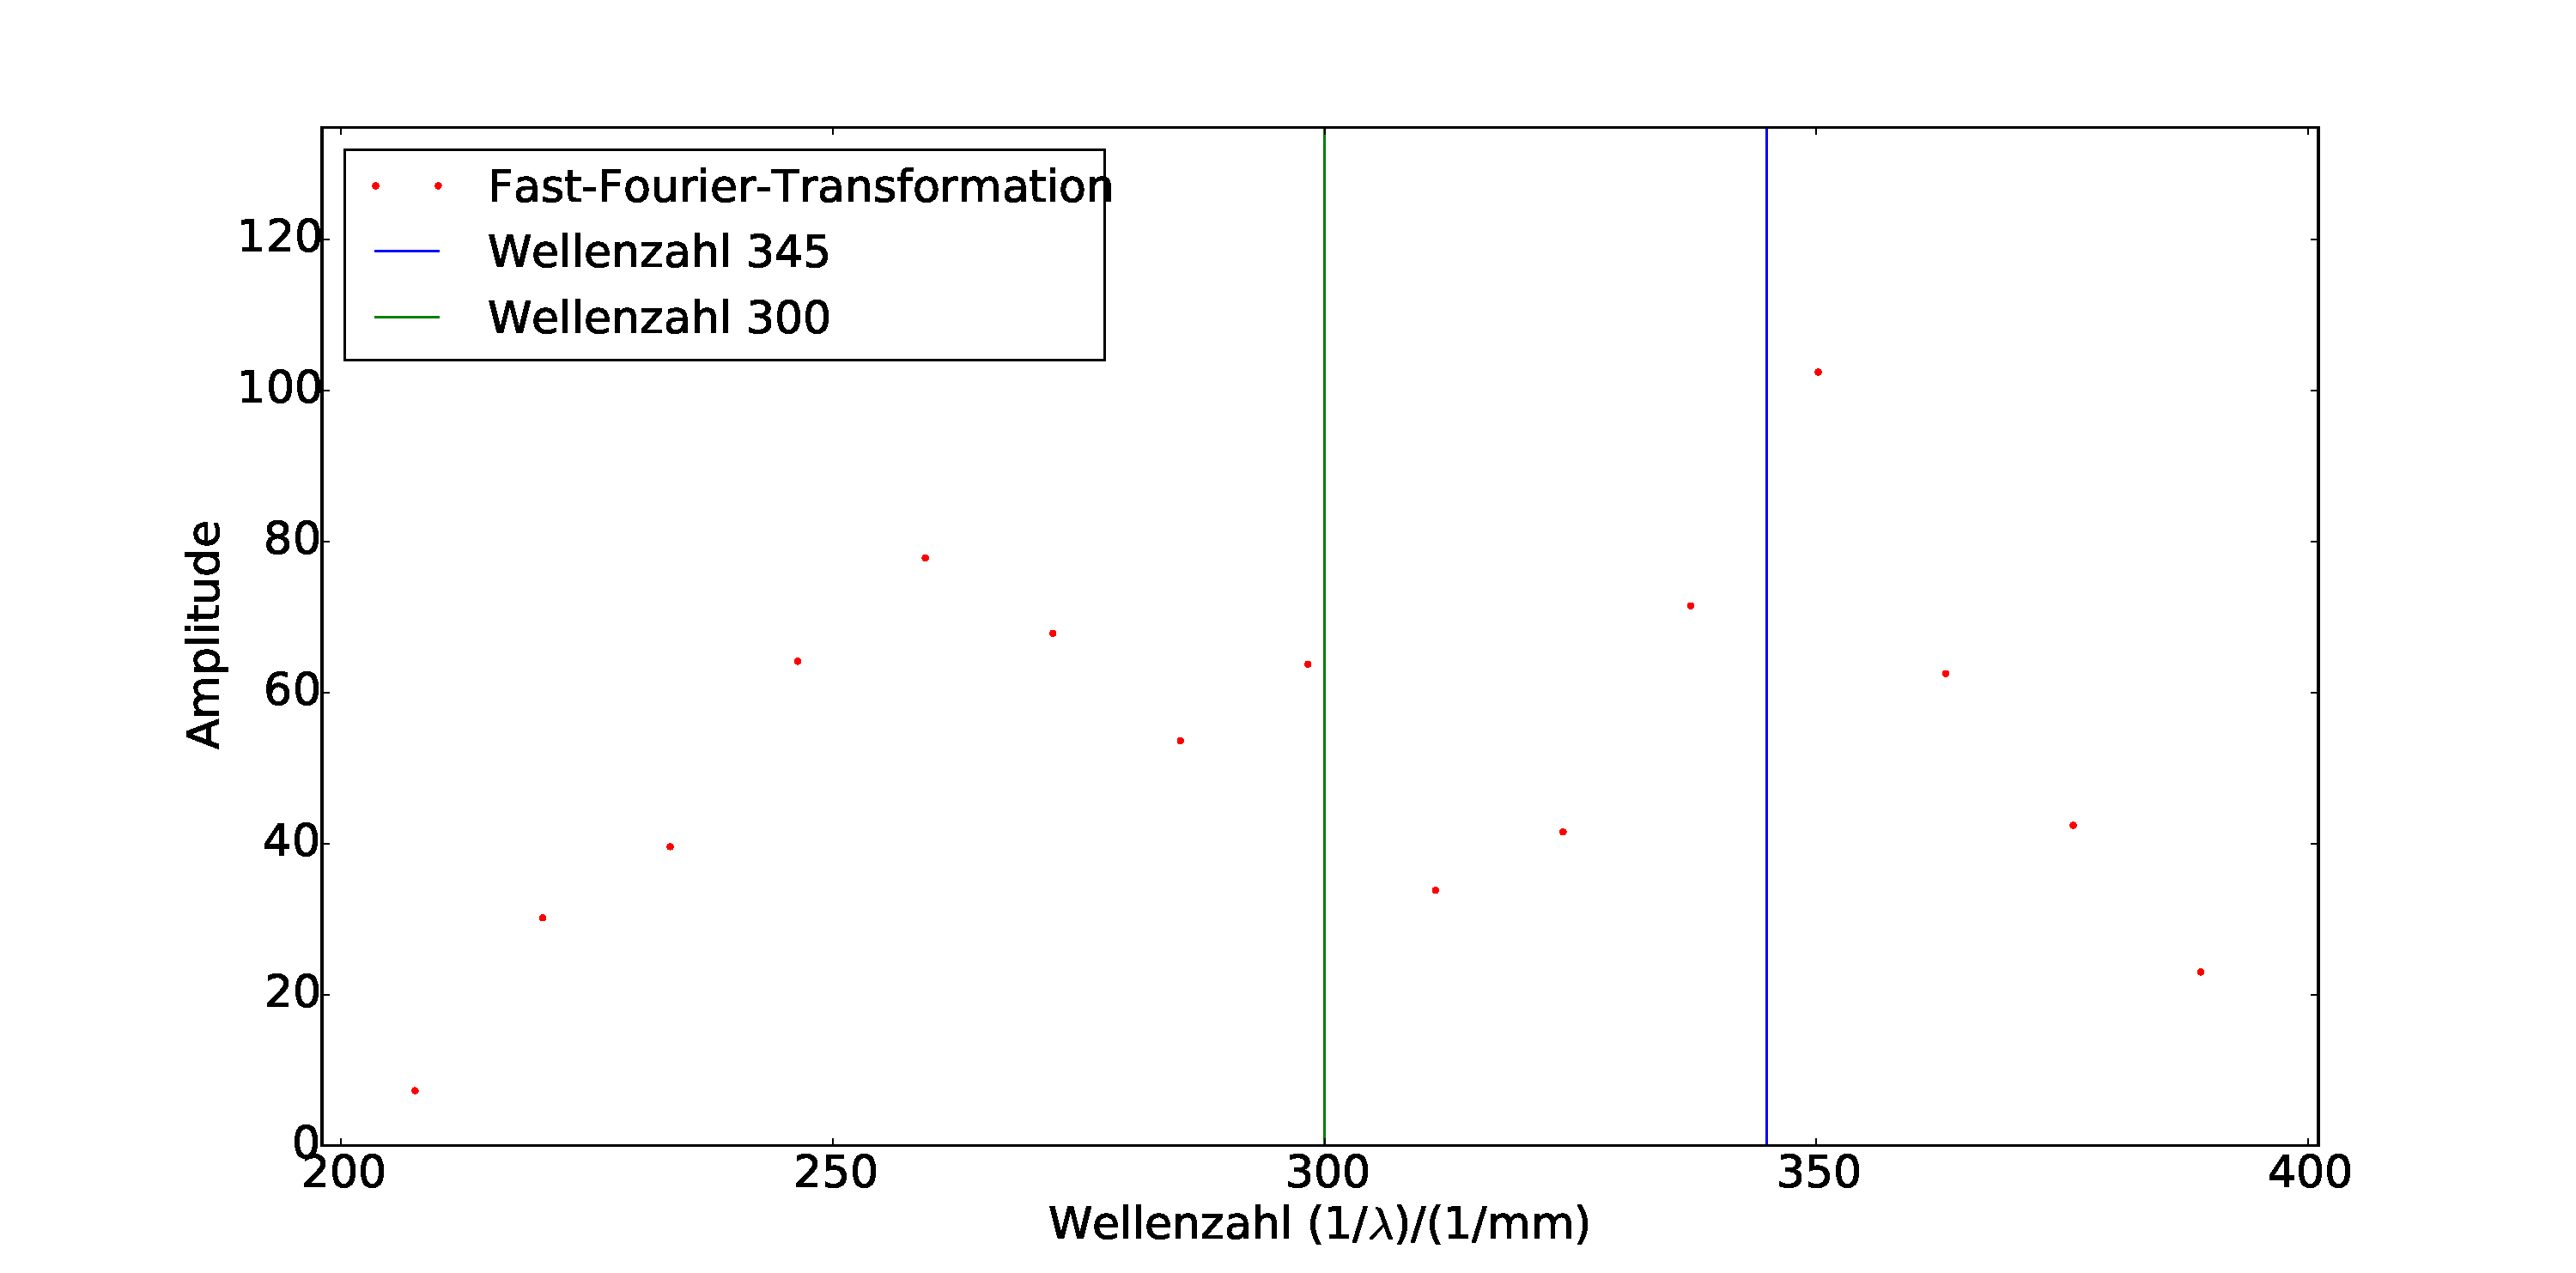
\includegraphics[scale = 0.19, clip = true, trim = 3cm 0cm 3cm 0cm]{Wellenzahlen200-400FiltermitFenster(0,5*(1-cos))}
\caption{Diskrete Fouriertransformation des Filterinterferogramms f�r Wellenzahlen ($1/\lambda$) von \SI{200}{$\frac{1}{mm}$} bis \SI{400}{$\frac{1}{mm}$} mit Fensterfunktion\\$f(x)=(\frac{1-\cos(\frac{2 \pi x}{L})}{2})$}
\label{fig:fftfilterinterferogramm_k_1}
\end{subfigure}
\hspace{0.02\textwidth}
\begin{subfigure}[t]{0.49\textwidth}
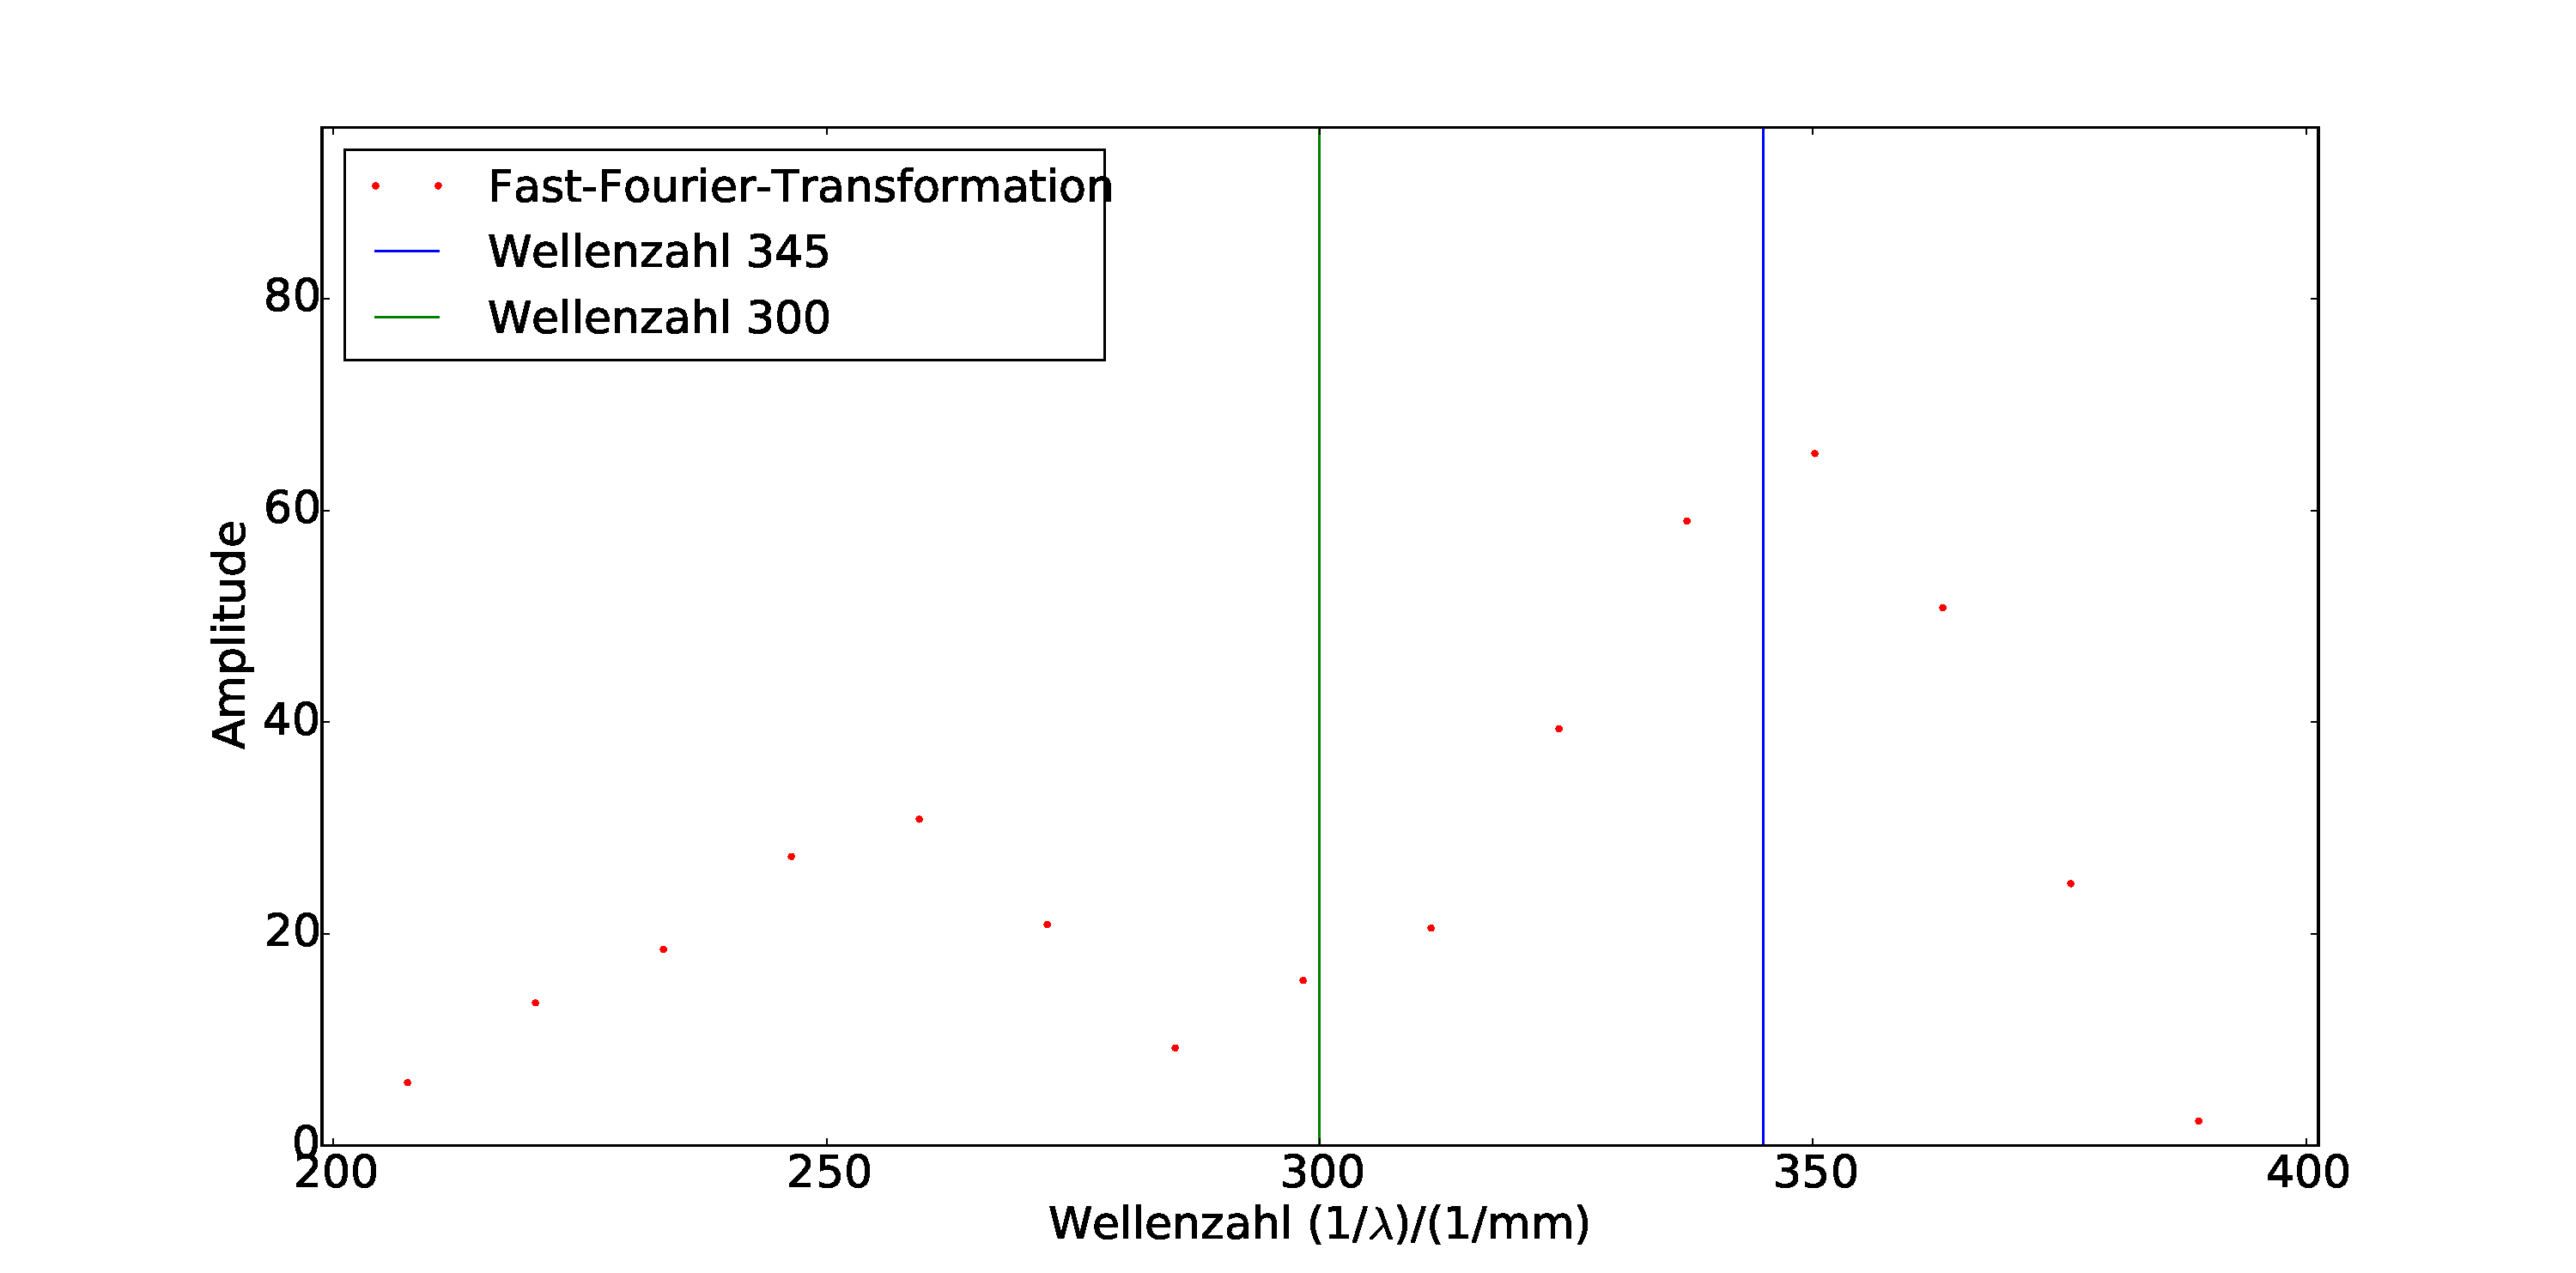
\includegraphics[scale = 0.19, clip = true, trim = 3cm 0cm 3cm 0cm]{Wellenzahlen200-400FiltermitFenster(0,5*(1-cos))**4}
\caption{Diskrete Fouriertransformation des Filterinterferogramms f�r Wellenzahlen ($1/\lambda$) von \SI{200}{$\frac{1}{mm}$} bis \SI{400}{$\frac{1}{mm}$} mit Fensterfunktion\\$f(x)=(\frac{1-\cos(\frac{2 \pi x}{L})}{2})^4$}
\label{fig:fftfilterinterferogramm_k_4}
\end{subfigure}
\end{figure}
Man sieht, dass der gr��te Peak, mit der Fensterfunktion $f(x)=(\frac{1-\cos(\frac{2 \pi x}{L})}{2})^k$ ($k=1,4$) bei einer Wellenzahl von \SI{345(2)}{$\frac{1}{mm}$} liegt, was einer Wellenl�nge von \SI{2,90(2)}{$\mu$m} entspricht. Diese stimmt mit der manuell bestimmten Wellenl�nge von \SI{2,91(5)}{$\mu$m} zu \SI{99,7}{\percent} �berein. Dieses Ergebnis spricht f�r die Konsistenz der manuellen Messung.